% il existe plusieures classes de documents
% pour des documents plus longs, vous pouvez utiliser
\documentclass[a4paper,12pt,twoside]{article}


% vous pouvez changer les paramètres : voici les options dispoinibles :
% - a4paper
% - fancysections
% - notitlepage ou titlepage
% - onside ou twoside selon si vous voulez l'imprimer en recto-verso ou en recto
% - sectionmark
% - chaptermark (pour les 
% - pagenumber
% - enmanquedinspiration
% en cas de doutes, pas de doutes, la documentation est sur :
%  https://gitlab.binets.fr/typographix/polytechnique/-/blob/master/source/polytechnique.pdf
\usepackage[a4paper,  fancysections,  titlepage]{polytechnique}
\usepackage[english]{babel}
\usepackage[utf8]{inputenc}
\usepackage[T2A,T1]{fontenc}
\usepackage{blindtext}
\usepackage[hidelinks]{hyperref}
\usepackage{amsmath, amssymb}
\usepackage{amsthm}
\usepackage{algorithm2e}
\usepackage{graphicx}
\newtheorem{definition}{Definition}
\newtheorem{example}{Example}
\newtheorem{theorem}{Theorem}
\usepackage{subcaption} 
\usepackage{nicefrac}

\def\dsqcup{\sqcup\mathchoice{\mkern-7mu}{\mkern-7mu}{\mkern-3.2mu}{\mkern-3.8mu}\sqcup}

% nous avons défini deux commandes :
\newcommand{\code}[1]{%
    \mbox{\ttfamily%
        \detokenize{#1}%
    }%
}

\newcommand{\resultat}[1]{%
    \quad \rightsquigarrow \quad #1%
}

\author{Badiss Ben Abdallah, Gaetan Ecrepont, Samson Gourevitch}
\title{Volatility Estimation Using High-Frequency Financial Data}
\subtitle{Research Report}%
% pour changer de logo, ajoutez l'image dans un fomat PDF
% ou image en la glissant à droite et remplacez typographix
% par le nom de l'image, si vous ne voulez pas de logo, 
% supprimze la ligne. 
%\logo{typographix}


\begin{document}
	\maketitle 
	\tableofcontents

\newpage

% abstract
 \begin{abstract}
    In this paper we will tackle the issue of volatility estimation when dealing with high-frequency financial data. We will use EUR/USD tick-by-tick forex data to test our models. We will first discuss ARCH and GARCH modeling of forex time series. Then we will look into non-naive high-frequency integrated variance estimators. Finally we will show how point processes can be used to model high-frequency price dynamics.
\end{abstract}


% introduction
\section*{Introduction}
    
    The increasing availability of quality high-frequency financial data has enabled better modeling of intraday asset prices dynamics. Although diffusion models are rather accurate at daily timescales, they fail to reproduce some of the stylized facts exhibited by high-frequency price data such as the divergence of the signature plot at very short timescales \cite{signature_plot} or the Epps effect \cite{epps}.
    
    In particular, estimating the volatility of an asset's price process at very high frequency is hard because of the discrete nature of price variations and the impact of microstructure noise \cite{bacry}.

    We will first review stylized facts exhibited by high-frequency financial data in Section \ref{section-badiss}. Then we will study different estimators of variance at short timescales in Section \ref{section-gaetan}. Finally, in Section \ref{section-samson} we will use point processes to model price dynamics.

\newpage
% first section
\section{Badiss} \label{section-badiss}

\newpage

\section{Estimating volatility at short timescales} \label{section-gaetan}
Because of the idiosyncrasies of high-frequency financial data, often subsumed under the umbrella term \textit{microstructure noise}, estimating the volatility of the price process at short timescales is an arduous task. In theory, a higher sampling rate should increase the estimator's accuracy because of the larger number of data points. However, when taking into account the fact that the observed price is a noisy version of the latent price, one quickly realizes that naive volatility estimators are doomed at high frequencies.

In this section, we will first explain why naive estimators diverge at high frequency, then we will show that low-frequency estimators actually fare better. We will finally describe an unbiased volatility estimator proposed in \cite{princeton} which takes the best of both world between high-frequency and low-frequency. All proofs have been omitted and can be found in \cite{princeton}.
\subsection{Naive High-Frequency Estimator}
Let $S_t$ be the price process of a security and suppose that $X_t=\log S_t$ follows an Itô process: $$dXt = \mu_t dt + \sigma_t dB_t$$ where $B_t$ is a standard Brownian motion.
We seek to estimate the integrated variance of the process $X_t$ over the time interval $[0,T]$, i.e. $IV=\int_0^T\sigma_t^2 dt$. A natural estimator is to use the sum of squared returns, also known as realized variance: $$\hat{IV}_\text{naive}=\sum_{t_i}(X_{t{i+1}}-X_{t_i})^2$$
Indeed, we know by stochastic calculus that this estimator converges towards $IV$ almost surely as the sampling frequency of the $t_i$ goes to infinity.

However, it has been shown empirically that this naive estimator behaves poorly at higher frequencies, typically under a five minutes, again because of microstructure effects. A simple way to understand this phenomenon is to incorporate \textit{observation error} in the process. That is, we observe $Y_{t_i}=X_{t_i}+\epsilon_{t_i}$ instead of the latent process $X_t$. In this model, the $\epsilon_{t_i}$ are independent centered random variables with finite variance $\mathbb{E}[\epsilon^2]=S^2$ accounting for the contamination of the latent price by microstructure effects. Within this framework, we now have $$\hat{IV}_\text{naive} \xrightarrow[]{L^1}IV + 2nS^2$$ where $n$ is the total number of points sampled. Since $IV$ is bounded, we see that increasing the sampling frequency increases the bias of the estimator and indeed it diverges linearly with $n$ as the sampling frequency increases. Thus, when using ultra high-frequency data e.g. tick-by-tick, $2nS^2 \gg IV$ such that the naive estimator becomes entirely irrelevant. In fact, when $2nS^2 \gg IV$, $IV_\text{naive}$ estimates the microstructure noise $2nS^2$ instead of the integrated variance $IV$.
\subsection{Improved Low-Frequency Estimator}
One easy way to deal with the poor performance of the naive estimator at high frequencies is to sample the data sparsely. For instance, if we have second-by-second data, we can sample every 300 points bring down the sampling frequency to 5 minutes.
In this case, we can show that $$\hat{IV}_\text{sparse} \approx^{\mathcal{L}} IV + 2n_\text{sparse}S^2 + \big[ 4n_\text{sparse}\mathbb{E}[\epsilon^4]+\frac{2T}{n_\text{sparse}}\int_0^T \sigma_t^4 dt \big]^{1/2}N(0,1)$$
In this setting, we see that reducing $n_\text{sparse}$ effectively reduces the bias of the naive estimator. If we also take into account the variance of the estimator, we can choose $n_\text{sparse}$ to minimize the MSE of the estimator, yielding $$n_\text{sparse}^* = \big( \frac{T}{4S^4}\int_0^T \sigma_t^4 dt \big)^{1/3}$$

\subsection{Subsampling and averaging}
Although the above low-frequency approach reduces the bias of the integrated variance estimator, it is still frustrating because it only uses a small portion of the available data. For instance, subsampling every 5 minute on second-by-second data amounts to discarding 299 observations every 300. A better approach is to separate the $n$ observations into $K$ low-frequency bins and then compute $\hat{IV}_\text{sparse}^{(i)}$ over each bin $B_i$ for $1\leq i \leq K$. We then consider the average $$\hat{IV}_\text{sparse}^\text{avg}=\frac{1}{K}\sum_{i=1}^K \hat{IV}_\text{sparse}^{(i)}$$
The most natural way to build the bins is to choose a low sampling frequency such as 5 minutes, and then choose $B_1$ to be the first observation in every 5-min interval, $B_2$ to be the second observation in every 5-min interval, etc. as illustrated in Figure \ref{fig-bins}.

\begin{figure}[h]
    \centering
    \includegraphics[width=0.8\textwidth]{img/bins.png}
    \caption{Building $K=5$ bins out of 1-min sampled data.}
    \label{fig-bins}
\end{figure}

Thus, averaging over $K$ bins of average size $\bar{n}$, one can show that $$\hat{IV}_\text{sparse}^\text{avg} \approx^{\mathcal{L}} IV + 2\bar{n}S^2 + \big[ 4\frac{\bar{n}}{K}\mathbb{E}[\epsilon^4]+\frac{4T}{3\bar{n}}\int_0^T \sigma_t^4 dt \big]^{1/2}N(0,1)$$
We see that $\hat{IV}_\text{sparse}^\text{avg}$ is still a biased estimator, but the bias $2\bar{n}S^2$ now scales with the average size of the bins $\bar{n}$ instead of the total number of points $n$, and because $\bar{n}=\frac{n}{K}<n$ the bias effectively diminishes as $K$ increases. Again, if we look at both bias and variance, we can optimize $\bar{n}$ for the MSE of $\hat{IV}_\text{sparse}^\text{avg}$, and we then set $K^*=\frac{n}{\bar{n}^*}$ as the optimal numbers of bins. In this case we can show that $$\bar{n}^*=\big( \frac{T}{6S^4} \int_0^T \sigma_t^4 dt \big)^{1/3}$$

\subsection{Combining High-Frequency with Low-Frequency}
Although the sparse-average estimator uses all the data while avoiding the high-frequency sampling issue, it is still a biased estimator, with bias $2\bar{n}S^2$. However, recall that the high-frequency naive estimator measures precisely the microstructure-induced bias $2nS^2$. Thus, we can use the high-frequency estimator $\hat{IV}_\text{naive}$ to de-bias the low-frequency estimator $\hat{IV}_\text{sparse}^\text{avg}$ by defining $$\hat{IV}_\text{best}=\hat{IV}_\text{sparse}^\text{avg}-\frac{\bar{n}}{n}\hat{IV}_\text{naive}$$
In this setting, if the number of bins is selected as $K=cn^{2/3}$, one can show that
$$\hat{IV}_\text{best} \approx^{\mathcal{L}} IV + n^{-1/6}\big[ \frac{8}{c^2}S^4 + c\frac{4T}{3}\int_0^T \sigma_t^4 dt \big]^{1/2}N(0,1)$$
Although this estimator converges at rate $n^{-1/6}$ only, it is unbiased and allows for sampling at arbitrarily high frequencies. In addition, $c$ can be optimized for MSE, yielding $$c^*=\big( \frac{T}{12S^4}\int_0^T \sigma_t^4 dt \big)^{1/3}$$

\subsection{Assessing estimator performance on synthetic data}
We will now compare the performance of our four estimators, from worse to best: $\hat{IV}_\text{naive}$, $\hat{IV}_\text{sparse}$, $\hat{IV}_\text{sparse}^\text{avg}$ and $\hat{IV}_\text{best}$.
To do so, we will use synthetic data generated using the Heston stochastic volatility model \cite{heston}. This way, we will know the true value of the integrated variance $IV=\int_0^T \sigma_t^2 dt$ and we will be able to compare it to the estimated value $\hat{IV}$ for each estimator.
Following the Heston model, the asset price $S_t$ will obey the following dynamic
$$dS_t = S_t\sigma_t dB_t^S$$
$$d\sigma_t^2 = \kappa(\theta-\sigma_t^2)dt + \sigma \sigma_t\delta dB_t^\sigma$$
Note that we set $\mu_t=0$ for the sake of simplicity. In addition, the two Brownian motions $B^S$ and $B^\sigma$ should be negatively correlated to account for the so-called \textit{leverage effect}, which states that negative returns tend to increase future volatility. Note that the variance $\sigma_t^2$ follows a CIR process and if the Feller condition $2\kappa \theta > \sigma^2$ are met, then the variance remains positive and cannot reach zero. In this setting, $\theta$ is the long-term variance equilibrium while $\kappa$ is the pullback strength towards that equilibrium. Finally, $\sigma$ is the volatility of the CIR process and as such it can be thought of as the volatility of the volatility, or \textit{vol of vol}.

Following \cite{liquidity}, we use parameters $\sigma=0.5$, $\kappa=5$, $\theta=0.1$ and $\rho=-0.3$ for the correlation between $B^S$ and $B^\sigma$. We also set $S=0.001$ the standard deviation of the microstructure noise, such that $\mathbb{E}[\epsilon^2]=S^2$. We also set $\sigma_0^2=\theta=0.1$ as the initial variance.

We use an Euler integration scheme to simulate our stochastic system, and since we want high-frequency data we use a time step $dt=1s$. We also set $T=24h$, such that we have a total of $n=86400$ samples.

In this setting, the naive high-frequency estimator will use a 1-second sampling frequency i.e. the highest possible, while the naive low-frequency estimator will use a 5-minute sampling frequency, i.e. 1 observation kept every 300. The sparse-average estimator and the best estimator will both use $K=300$ bins, such that the resulting per-bin sampling frequency is $86400/300=288s$ i.e. one observation every 2min48s.

The simulation protocol is as follows:
\begin{enumerate}
    \item we generate $M$ independent price paths using the Heston model described above
    \item for each price path $X^{(i)}$, we compute the integrated variance as the discrete integral of the $(\sigma_t^{(i)})^2$, and we compute the four estimates $\hat{IV}_\text{naive}^\text{HF}$, $\hat{IV}_\text{naive}^\text{LF}$, $\hat{IV}_\text{sparse}^\text{avg}$ and $\hat{IV}_\text{best}$
    \item for each estimator we plot the histogram of the relative error $\frac{\hat{IV}-IV}{IV}$
\end{enumerate}

The resulting histograms are given in Figure \ref{fig-hists}. As expected, we see that the high-frequency naive estimator behaves extremely poorly, with a relative approximation error consistently above 500. The low-frequency estimator is two orders of magnitude better in terms of performance but is still highly biased, with a relative approximation error consistently greater than 1.5. The sparse-average estimator is only slightly better than the low-frequency naive estimator, with a similar positive bias but lower variance overall. Finally, the best estimator is the only unbiased estimator and also has the lowest variance, making it far better than the preceding estimators. In our Monte Carlo simulation, we find that the relative error $\frac{\hat{IV}_\text{best}-IV}{IV}$ is centered with a standard deviation of about 0.07, meaning that the relative error is below 14\% in 95\% of cases.

Thus, we can conclude that $\hat{IV}_\text{best}$ is a satisfying estimator of integrated variance which has moderate variance thanks to its low-frequency part and no microstructure-induced bias thanks to its high-frequency part.

\begin{figure}[h]
    \centering
    \includegraphics[width=0.8\textwidth]{img/IV_estimators_hist.png}
    \caption{Histogram of the relative error $\frac{\hat{IV}-IV}{IV}$ for the four estimators proposed using Monte Carlo simulations with $M=1000$.}
    \label{fig-hists}
\end{figure}

\subsection{Implementation on tick-by-tick forex data}
In this last subsection, we will look at high-frequency, tick-by-tick forex data for the EUR/USD pair obtained from TrueFX. We will first measure integrated variance using the naive estimator $\hat{IV}_\text{naive}$ at various frequencies to check that our estimations do indeed diverge as the sampling frequency goes to infinity. We will then measure integrated variance using the best estimator $\hat{IV}_\text{best}$ and compare the results.

To avoid the abnormal spread occurring on forex between 22:00 and 22:30 (because of large banks performing their daily IT maintenance during this time slot), we will look at just 23 hours of non-stop EUR/USD data collected from 02/04/2024 18:00 EST to 02/05/2024 17:00 EST. Our dataset is tick-by-tick data containing only the best bid and best ask at a given time. We have a total of 681,912 ticks, representing an average of 8.24 ticks/s. We could define $S_t$ to be the logarithm of the mid price $\text{mid}=\frac{\text{ask}+\text{bid}}{2}$ but in practice this leads to an artificial reduction of volatility (since we're averaging). Thus, we will take the logarithm of the best bid for $S_t$. Using the best ask yields identical results.

Our experiment protocol is the following:
\begin{enumerate}
    \item we define a range of sampling frequencies from $\tau=100ms$ to $\tau=20s$ using $100ms$ intervals
    \item for each of $\tau$, we resample $S_t$ to this frequency. [note that when a resampling bin has several ticks we take the first (i.e. earliest) one, and when a resampling bin has no ticks we use forward fill (i.e. the fill the value with the latest value available)]
    \item we estimate integrated variance over our whole dataset using the naive estimator and the best estimator, both sampling at frequency $\tau$ [note that for the sake of completeness we use $K=10,100,1000$ for the best estimator]
    \item we plot $\big(\tau,\hat{IV}(\tau)\big)$ for each estimator
\end{enumerate}

\begin{figure}[h]
    \centering
    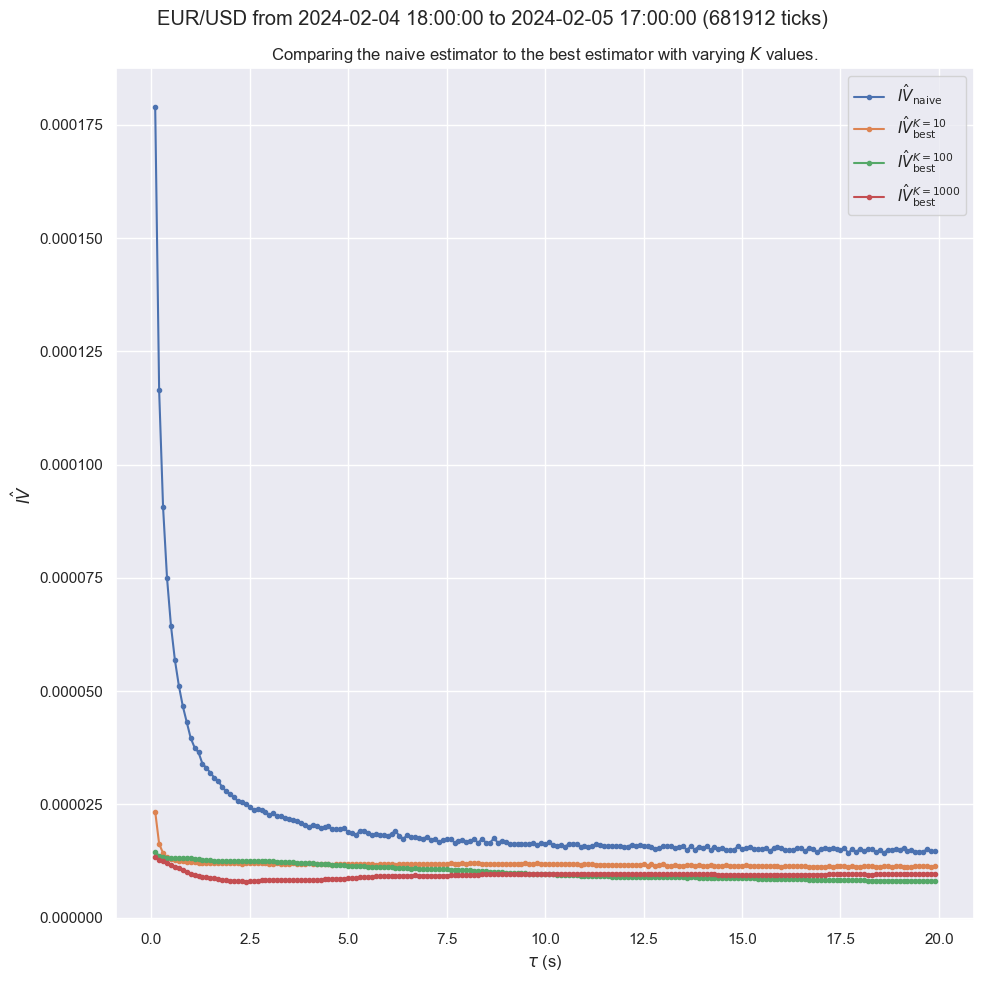
\includegraphics[width=0.8\textwidth]{img/output_iv_forex.png}
    \caption{Integrated variance estimated using naive estimator and best estimator at various frequencies.}
    \label{fig-IV-forex}
\end{figure}

The results are illustrated in Figure \ref{fig-IV-forex}. As expected, the naive estimator diverges at high sampling frequencies, as early as $\tau\sim10s$. On the contrary, the best estimator remains stable at higher frequencies for all values of $K$, though for $K=10$ we see a small bias at the highest sampling frequency ($\tau=100ms$). Interestingly, the best estimators for $K=100$ behave slightly differently, with the $\hat{IV}_\text{best}^{K=100}$ monotonously increasing as $\tau$ decreases, whereas $\hat{IV}_\text{best}^{K=1000}$ remains very stable up to $\tau\sim10s$ then decreases and reaches a minimum at around $\tau\sim2s$ and then increases again. In this case we obviously do not know the integrated variance so we cannot be sure which of these two estimators is more accurate.


\section{Samson} \label{section-samson}
\subsection{Modeling the price by a Hawkes process}

Up until now, we have modeled the so-called micro-structure noise (as it is often done in litterature) with the introduction of a latent price and an additive noise. 
However, although this approach can give interesting results, it doesn't quite reproduce the high frequency effects that we are interested in. In this report, we will focus on one specific effect which affects the shape of the signature plot. This signature plot is simply the plot of the realized volatility against the sampling frequency.

Add an image of the signature plot.

One the the problems of the additive noise model is that it doesn't really give insight into the nature of this noise and its micro-structure properties and the introduction of a noise at high frequency may seem a bit artificial.

To remediate those issues, we introduce a new dynamic which explains price movements using mutually exciting Hawkes processes.

Let $X(t)$ be the price of our asset, $N_1(t)$ and $N_2(t)$ two point processes that represents the sum of positive and negative price jumps up until the time $t$. Then we have : \begin{equation} X(t) = N_1(t) - N_2(t) \end{equation}. 

The idea is that $N_1(t)$ and $N_2(t)$ are mutually exciting at short time scales. This means that at high frequency, when the price goes up a little bit, it tends to go down right after and thus we model our mean reverting property. At longer time scales, the model should behave as a brownian motion to match the Black-Scholes model. This is indeed the case if $N_1(t)$ and $N_2(t)$ are independent Poisson processes with intensity $\mu$ for instance.
Indeed, in this case 

% Add explanations
the characteristic function of $N_1(t) - N_2(t)$ is given by $\exp(-2\mu + \mu(\exp(it) + \exp(-it)) = \exp(2\mu(cos(t) - 1)$. Therefore 

\begin{equation}
\lim_{t \to \infty} \frac{1}{\sqrt{T}}X(tT) = \sqrt{2\mu}B(t)
\end{equation}

where $B(t)$ is a Brownian motion.

This approach can thus give a unified view of the asset's price behaviour while reproducing (as we will show later) the effects we observe at both high and low frequencies.

These mutually exciting processes can be naturally modelled by Hawkes processes in order to introduce those time scale differences (which will be modeled by the shape of the kernels). Let $\lambda_1$ and $\lambda_2$ be the intensities of $N_1$ and $N_2$. 

The mean reverting property we aim for suggest to set the self-exciting kernels to 0 and simply keep the base excitations as well as the cross exciting kernels. Therefore, we have 

\begin{equation} \lambda_i = \mu_i + \int_{-\infty}^{t} \phi_{ij}(t-u)dN_j(u), i \in {1, 2}.
\end{equation}

As the situation appears to be symmetric if the price goes down or up (it may not be completely true but we make this approximation), we take $\phi_1 = \phi_2 = \phi$. As it is done in (insert article), we use exponential kernel for simplicity and because this can easily relate to the time scale we are considering. Therefore, we have $\phi(t) = \beta \cdot \exp(-\alpha t)$ where $\alpha, \beta \in \mathbb{{R^{+}}^*}$.

To make sure this approach is sensible, we can compare the plots of real tick data versus data generated by our model. 

Insérer les deux plots

We see that they look similar. Although this is no proof, it is reassuring that our model gives similar outputs if we want to fit it to real data later.

\subsection{Explaining the signature plot}

We introduce an estimator of the volatility at the frequency $\frac{1}{\tau}$  

\begin{equation}
    \hat{C}(\tau) = \frac{1}{T}\sum_{n=0}^{\nicefrac{T}{\tau}}(X((n+1)\tau) - X(n\tau))^2
\end{equation}

\subsection{Fitting the model on real data}


// pas besoin de conclu imo

\begin{thebibliography}{}
    \bibitem{bacry}{Bacry, E. \textit{Modeling microstructure noise with mutually exciting point processes} (2018).}
    \bibitem{princeton}{Zhang, L. et al. \textit{A Tale of Two Time Scales: Determining Integrated Volatility With Noisy High-Frequency Data} (2018).}
    \bibitem{signature_plot}{Hansen, P. et al. \textit{Realized Variance and Market Microstructure Noise} (2004).}
    \bibitem{epps}{Epps, T. W. \textit{Comovements in stock prices in the very short run} (1979).}
    \bibitem{heston}{Heston, S. \textit{A closed-form solutions for options with stochastic volatility} (1993).}
    \bibitem{liquidity}{Aït Sahalia Y. \textit{High frequency market microstructure noise estimates and liquidity measures} (2009).}
    
    
\end{thebibliography}	
\end{document}